
%\chapter*{A brief introduction to quantum field theory in curved spacetimes: Introduction to the Unruh and Hawking effects}[Intro to the Unruh and Hawking effects]
%\label{chap:introUnruh}

\chapter{Population bound effects on non-inertial bosonic correlations\footnote{E. Mart\'in-Mart\'inez, J. Le\'on. Phys. Rev. A, 81, 052305 (2010}}\label{boundedpop}
\markboth{Chapter 6. Non-inertial bosonic correlations: Population bound effects  }{\rightmark}


We have seen before, studying different fermionic fields and for different kinds of states, that the Fock space dimension does not play a role in fermionic entanglement behaviour in non-inertial frames. In this chapter we will analyse the effects of artificially bounding the occupation number of the modes of a bosonic field while conserving Bose-Einstein-like statistics. Doing that we will be able to study from the bosonic perspective if the Hilbert space dimension has any relevance in non-inertial entanglement behaviour.

As we did in previous chapters, we will consider once again a bipartite system (Alice-Rob), in which one of the partners (Rob) is undergoing a uniform acceleration and therefore describing the world which Rindler coordinates. As pointed out in \cite{AlsingSchul} and the previous chapter, there are 3 possible bipartitions that can be considered when analysing entanglement in this setting; 1) The entanglement of the inertial observer with field modes in Rindler's region I (Alice-Rob, AR), 2) The entanglement of the inertial observer with field modes in Rindler's region II (Alice-AntiRob, $\text{A}{\bar{\text{R}}}$) and 3) The entanglement between modes in regions I and II of the Rindler spacetime (Rob-AntiRob $\text{R}{\bar{\text{R}}}$). Partitions AR and $\text{A}{\bar{\text{R}}}$ are especially important as these are the partitions in which classical communication is allowed (we will refer to them as CCA bipartitions from now on).

In chapter \ref{etanthrough} we have explored the radical differences between fermionic and bosonic entanglement behaviour in the presence of Rindler and event horizons, showing that the real cause of these differences is fermionic/bosonic statistics. This contradicts the naive argument that the differences come from the finite dimensional nature of the fermionic Hilbert space for each frequency as opposed to the built-in infinite dimension of the Fock space for bosons.

In an attempt to settle down the discussion about what effects are influenced by the dimension of the Hilbert space and which ones are not, we are going to study a finite dimensional analog to bosonic fields with a limited dimension of each frequency Fock space. This means engineering a method to impose a maximum occupation number $N$ in each scalar field frequency mode. The construction of a finite dimensional scalar field state for a non-inertial observer can be problematic, thus it is an issue which will need to be tackled in order to conduct the proposed analysis.

We will present results about entanglement of the CCA bipartitions that will strengthen the argument discussed in previous chapters on the capital importance of statistics in the phenomenon of entanglement degradation due to the Unruh effect. Specifically we will prove that the behaviour is fundamentally independent of the Fock space dimension. However, bosonic entanglement for AR is slightly sensitive to Fock space dimension variation, in opposition to what happens with fermions. 

We shall point out that those variations strongly oppose once again what is said in previous literature in which it is argued that the Unruh decoherence degrades the entanglement quicker as the dimension of the Hilbert space is higher. Instead, we will show that quantum correlations can be more or less quickly degraded for different dimensions depending on the value of the acceleration. This completely banishes the former argument. 

Furthermore, we will show remarkable results concerning correlations between modes in Rindler regions I and II. We will see how they are ruled by both statistics and Hilbert space dimension. There are differences and similarities between fermions and bosons concerning correlations $\text{R}{\bar{\text{R}}}$. We will analyse the different bosonic cases comparing them with their Fock space dimension fermionic analogs, in order to comprehend the relative importance of dimensionality and statistics in the behaviour of such correlations.

We will also show how classical correlations between AR and $\text{A}{\bar{\text{R}}}$ are affected by the bound on the occupation number. Specifically we will show that the effect of imposing a finite dimensional Fock space affects the conservation law for mutual information found in previous works. We will compare this with the fermionic cases and will prove some results about mutual information to be completely universal.

\section{Limiting the occupation number}\label{sec3}

The Minkowski vacuum state for a $\omega$-frequency mode of a scalar field seen from the perspective of an accelerated observer is
\begin{equation}\label{scavacinfm5}
\ket{0_\omega}=\frac{1}{\cosh r}\sum_{n=0}^\infty \tanh^n r \ket{n}_{\text{I}}\ket{n}_{\text{II}}.
\end{equation}
We will drop the frequency label as we will study single Unurh mode states as we did in previous chapters.

The Minkowskian Unruh one particle state results from applying the creation operator to the vacuum state. Its translation to the Rindler basis is
\begin{equation}\label{unoinfm5}
\ket{1}_\text{U}=\frac{1}{\cosh^2 r}\sum_{n=0}^{\infty} \tanh^n r \,\sqrt{n+1}\ket{n+1}_{\text{I}}\ket{n}_{\text{II}}.
\end{equation} 	
Now we will consider the following maximally entangled state in the Minkowski basis
\begin{equation}
\label{entangledscainf}\ket{\Psi}=\frac{1}{\sqrt{2}}\left(\ket{0}\ket{0}+\ket{1}_\text{U}\ket{1}_\text{U}\right).
\end{equation}
This is a qubit state which is a superposition of the bipartite vacuum and the bipartite one particle state completely equivalent to that studied in chapters before. 

For our purposes we need to limit the dimension of the Hilbert space. To do so we are going to limit the maximum occupation number for the Rindler modes up to $N$.

If we want to go beyond qualitative effects and do a completely rigorous analysis we would run into important problems. Namely, we would not be able to normalise both states  \eqref{scavacinfm5}, \eqref{unoinfm5} simultaneously. In other words, the translation into the Rindler basis of the Minkowskian creation operator applied on the vacuum state would not preserve normalisation and it would be no longer true that applying the annihilation operator to the one particle state we recover the vacuum of the theory. Therefore the canonical quantisation rules of bosonic fields would be ill-defined (for instance, problems would appear when applying the commutator to the one particle state). As statistics is fundamental to explain the Unruh decoherence mechanism, a rigorous analysis would require that we consider the vacuum of our theory as expressed in \eqref{scavacinfm5} with an unbounded occupation number.

Alternately, we will define finite dimension analogs to the vacuum and one particle states
\begin{equation}\label{scavac}
\ket{0_N}_\text{U}=\frac{1}{\cosh r}\sum_{n=0}^N \tanh^n r \ket{n}_{\text{I}}\ket{n}_{\text{II}},
\end{equation}
\begin{equation}\label{uno}
\ket{1_N}_\text{U}=\frac{1}{\cosh^2 r}\sum_{n=0}^{N-1} \tanh^n r \,\sqrt{n+1}\ket{n+1}_{\text{I}}\ket{n}_{\text{II}},
\end{equation} 	
in which we have cut off the higher occupation numbers and thus these two states are not exactly the vacuum of our theory and the first excitation. Instead, they could be understood as approximations in which Rob is not able to notice occupation numbers larger than $N$. Indeed this is a consistent approximation as the coefficients of higher $n$ become more and more smaller as $n$ grows. This simple construct allows us to consider a bounded occupation number along with bosonic statistics. Therefore we can now disentangle the statistical effects from the ones derived from the dimensionality of the Hilbert space. 

We will then consider the following entangled state in Minkowski coordinates
\begin{equation}
\label{entangledsca}\ket{\Psi}=\frac{1}{C_N(r)}\left(\ket{0}_\text{U}\ket{0_N}_\text{U}+\ket{1}_\text{U}\ket{1_N}_\text{U}\right),
\end{equation}
in which the one particle state and the vacuum for Rob are substituted by the bounded occupation number approximations\footnote{Alternatively, we could have considered a scalar field which is quantised with the following commutation rules: $[a,a^\dagger]=1+(N-1)\proj{N}{N}$. This field would share the same Rindler-Minkowski Bogoliubov coefficients than the standard scalar field and a maximum occupation number $N$ would be naturally imposed. Although the state normalisation of \eqref{scavac} and \eqref{uno} would have not been the same, \eqref{entangledsca} would have exactly the same form once it is normalised. The two approaches are equivalent for our purposes and produce the same results.}.

Notice that a factor $1/C_N(r)$ must now be included as our occupation number cutoff implies that $\ket{0_N}_\text{U}$ and $\ket{1_N}_\text{U}$ are not normalised. Its value is
\begin{equation}
C_N(r)=\sqrt{\braket{0_N}{0_N}_\text{U}+\braket{1_N}{1_N}_\text{U}},
\end{equation}
or, explicitly,
\begin{equation}
C_N(r)=\sqrt{2-\tanh^{2N}r\left(\tanh^2 r + 1 + \frac{N}{\cosh^2r}\right)}.
\end{equation}
In the limit $N\rightarrow\infty$, $C_{N}(r)\rightarrow\sqrt2$ recovering the standard scalar maximally entangled state \eqref{entangledscainf}.

Since we have restricted our whole Hilbert space to the sector of $N$ particles and no operation takes us out from it we can guarantee that Unruh decoherence will not affect higher occupation number modes.

The density matrix for the whole tripartite state, which includes modes in both sides of the horizon along with Minkowskian modes, is built from \eqref{entangledsca} changing to the Rindler basis for Rob
\begin{equation}\label{tripasca}
\rho^{A\text{R}{\bar{\text{R}}}}=\proj{\Psi}{\Psi}.
\end{equation}

The partial subsystems are obtained as usual
\begin{align}
\label{AR1}\rho^{AR}&=\tr_{\text{II}}\rho^{A\text{R}{\bar{\text{R}}}},\\*
\label{AAR1}\rho^{A\bar R}&=\tr_{\text{I}}\rho^{A\text{R}{\bar{\text{R}}}},\\*
\label{RAR1}\rho^{\text{R}{\bar{\text{R}}}}&=\tr_{\text{U}}\rho^{A\text{R}{\bar{\text{R}}}},
\end{align}
and the density matrix for each individual subsystem
 \begin{align}
\label{A1}\rho^{A}&=\tr_{\text{I}}\rho^{AR}=\tr_{\text{II}}\rho^{A\bar R},\\*
\label{R1}\rho^{R}&=\tr_{\text{II}}\rho^{\text{R}{\bar{\text{R}}}}=\tr_{\text{U}}\rho^{AR},\\*
\label{aR1}\rho^{\bar R}&=\tr_{\text{I}}\rho^{\text{R}{\bar{\text{R}}}}=\tr_{\text{U}}\rho^{\text{A}{\bar{\text{R}}}}.
\end{align}

The bipartite systems are characterized by the following density matrices
\begin{align}\label{rhoars1}
\rho^{AR}&=\!\left\{\sum_{n=0}^{N-1}\frac{\tanh^{2n}r}{\cosh^2r}\left[\proj{0n}{0n}+\frac{\sqrt{n+1}}{\cosh r}\Big(\proj{0n}{1\, n+1}\right.\nonumber+\proj{1\, n+1}{0n}\Big)\right.\nonumber\\*
&\left.\left.+\frac{n+1}{\cosh^2 r}\proj{1\,n+1}{1\,n+1}\right]+\frac{\tanh^{2N}r}{\cosh^2r}\proj{0N}{0N}\right\}\frac{1}{C_N(r)^2},
\end{align}
\begin{align}\label{rhoa-rs1}
\nonumber\rho^{A\bar R}&=\left\{\sum_{n=0}^{N-1}\frac{\tanh^{2n}r}{\cosh^2r}\left[\proj{0n}{0n}\!+\!\frac{\sqrt{n+1}}{\cosh r}\tanh r\Big(\!\ket{0\,n+1}\right.\bra{1 n}+\proj{1 n}{0\,n+1}\Big)\right.\nonumber\\*
&\left.\left.+\frac{n+1}{\cosh^2 r}\proj{1n}{1n}\right]+\frac{\tanh^{2N}r}{\cosh^2r}\proj{0N}{0N}\right\}\frac{1}{C_N(r)^2},
\end{align}
\begin{align}\label{rhor-rs1}
\nonumber\rho^{\text{R}{\bar{\text{R}}}}&=\frac{1}{C_N(r)^2}\Bigg\{\sum_{\substack{n=0\\m=0}}^{N}\frac{\tanh^{n+m}r}{\cosh^2r}\proj{nn}{mm}\\
&+\sum_{\substack{n=0\\m=0}}^{N-1}\frac{\tanh^{n+m}r}{\cosh^4r}\sqrt{n+1}\sqrt{m+1}\proj{n+1\,n}{m+1\,m}\Bigg\},
\end{align}
where the bases are respectively
\begin{eqnarray}\label{barbolbasis}
 \ket{nm}&=&\ket{n^A}_{\text{U}}\ket{m^R}_{\text{I}},\\*
\ket{nm}&=&\ket{n^A}_{\text{U}}|m^{\bar R}\rangle_{\text{II}},\\*
\ket{nm}&=&\ket{n^R}_{\text{I}}|m^{\bar R}\rangle_{\text{II}}
\end{eqnarray}
for \eqref{rhoars1}, \eqref{rhoa-rs1} and \eqref{rhor-rs1}.

On the other hand, the density matrices for the individual subsystems \eqref{A1}, \eqref{R1},\eqref{aR1} are
\begin{equation}\label{Robpartial}
\rho^{R}=\frac{1}{C_N(r)^2}\sum_{n=0}^N\frac{\tanh^{2n}r}{\cosh^2r}\left[1+\frac{n}{\sinh^2r}\right]\proj{n}{n},
\end{equation}
\begin{equation}\label{ARobpartial}
\rho^{\bar R}=\frac{1}{C_N(r)^2}\left[\sum_{n=0}^{N-1}\frac{\tanh^{2n}r}{\cosh^2r}\left(1+\frac{n+1}{\cosh^2r}\right)\proj{n}{n}+\frac{\tanh^{2N}r}{\cosh^2r}\proj{N}{N}\right],
\end{equation}
\begin{equation}\label{AlicedeAliceRob}
\rho^{A}=\frac{1}{C_N(r)^2}\left(D^0_N(r)\proj{0}{0}+D^1_N(r)\proj{1}{1}\right),
\end{equation}
where
\begin{equation}\label{S1}
D^0_N(r)=\sum_{n=0}^N\frac{\tanh^{2n}r}{\cosh^2 r}=1-(\tanh r)^{2(N+1)},
\end{equation}
\begin{equation}\label{S2}
D^1_N(r)\!=\!\! \sum_{n=0}^{N-1}(n+1)\frac{\tanh^{2n}r}{\cosh^2 r} =1-\left(1+\dfrac{N}{\cosh^2 r}\right) \tanh^{2 N}\!r.
\end{equation}
Notice that $D^0_N(r)+D^1_N(r)=C_N^2(r)$ and consequently all the density matrix traces are 1 as it must be. As all the probability is within the modes that we are considering, all the possible `decoherence' is confined to the finite occupation number Hilbert space we are studying. We are not just taking part of the complete vacuum and one particle states losing probability in our approximation, instead we have artificially imposed that the Unruh effect will only excite every mode up to a maximum occupation number $N$.

As an effect of the imposition of the finite dimension $\rho_A\rightarrow\proj00$ as $a\rightarrow\infty$ for any finite $N$, but it tends to $\frac12(\proj00+\proj11)$ when $N\rightarrow\infty$ for all $a$. It is important to notice that both limits do not commute. The limit $N\rightarrow\infty$ should be taken first in order to recover the standard scalar field result.

\section{Analysis of correlations}\label{sec4}

In this section we will analyse the correlations tradeoff among all the possible bipartitions of the system. We will account for the entanglement by means of the negativity, and we will study the total correlations by means of the mutual information, which accounts for both classical and quantum. 


\subsection{Quantum entanglement}\label{negatsec}

We will study quantum entanglement for the three bipartitions in this settings. For this, we will use negativity as an entanglement measure. To compute  negativity we need the partial transpose of the bipartite density matrices \eqref{rhoars1}, \eqref{rhoa-rs1} and \eqref{rhor-rs1}, which we will notate as $\eta^{AR}$, $\eta^{A\bar R}$ and $\eta^{R \bar R}$  respectively.
\begin{align}\label{etaARs}
\eta^{AR}&=\!\left\{\sum_{n=0}^{N-1}\frac{\tanh^{2n}r}{\cosh^2r}\left[\proj{0n}{0n}+\frac{\sqrt{n+1}}{\cosh r}\Big(\proj{0\,n+1}{1\, n}\right.\nonumber+\proj{1 n}{0\,n+1}\Big)\right.\nonumber\\*
&\left.\left.+\frac{n+1}{\cosh^2 r}\proj{1\,n+1}{1\,n+1}\right]+\frac{\tanh^{2N}r}{\cosh^2r}\proj{0N}{0N}\right\}\frac{1}{C_N(r)^2},
\end{align}
\begin{align}\label{etaAaRs}
\nonumber\eta^{A\bar R}&=\left\{\sum_{n=0}^{N-1}\frac{\tanh^{2n}r}{\cosh^2r}\left[\proj{0n}{0n}\!+\!\frac{\sqrt{n+1}}{\cosh r}\tanh r\Big(\!\ket{0n}\right.\bra{1\, n+1}+\proj{1\, n+1}{0\,n}\Big)\right.\nonumber\\*
&\left.\left.+\frac{n+1}{\cosh^2 r}\proj{1n}{1n}\right]+\frac{\tanh^{2N}r}{\cosh^2r}\proj{0N}{0N}\right\}\frac{1}{C_N(r)^2},
\end{align}
\begin{align}\label{etaRaRs}
\nonumber\eta^{\text{R}{\bar{\text{R}}}}&=\frac{1}{C_N(r)^2}\Bigg\{\sum_{\substack{n=0\\m=0}}^{N}\frac{\tanh^{n+m}r}{\cosh^2r}\proj{nm}{mn}\\
&+\sum_{\substack{n=0\\m=0}}^{N-1}\frac{\tanh^{n+m}r}{\cosh^4r}\sqrt{n+1}\sqrt{m+1}\proj{n+1\,m}{m+1\,n}\Bigg\}.
\end{align}

In the following subsections we shall compute the negativity of each bipartition of the system.
 
\subsubsection{Alice-Rob Bipartition}


Apart from the diagonal elements corresponding to $\proj{00}{00}$ and $\proj{1N}{1N}$ (which form two $1\times1$ blocks themselves), the partial transpose of the density matrix $\rho^{A R} $ \eqref{etaARs} has a $2\times2$ block structure in the basis $\{ \ket{0\, n+1},\ket{1 n}\}_{n=0}^{N-1}$
\begin{equation}\label{blocks}
\frac{\tanh^{2n}r}{C(r)^2\cosh^2 r}
\left(\!\begin{array}{cc}
\tanh^2 r & \dfrac{\sqrt{n+1}}{\cosh r}\\
\dfrac{\sqrt{n+1}}{\cosh r} & \dfrac{n}{\sinh^2r}
\end{array}\!\right).
\end{equation}
Hence, the eigenvalues of \eqref{etaARs} are
\begin{align}
\nonumber\lambda^\pm_n&\!=\!\frac{\tanh^{2n} r}{2C_N(r)^2\cosh^2 r}\Bigg[\!\left(\frac{n}{\sinh^2r}+\tanh^2 r\right)\left.\!\pm\sqrt{\left(\frac{n}{\sinh^2r}+\tanh^2 r\right)^2\!+\frac{4}{\cosh^2 r}}\right]_{n=0}^{N-1}\!\!\!\!,\\*
\lambda_N&=\frac{1}{C_N(r)^2\cosh^2r};\qquad\qquad \lambda_{N+1}=\frac{N(\tanh r)^{2N-2}}{C_N(r)^2\cosh^4 r}.
\end{align}
Here, the notation $\displaystyle{|_{n=a_1}^{a_N}}$ means that $n$ takes all the integer values from $a_1$ to $a_N$.

Therefore the negativity for this bipartition is
\begin{equation}
\mathcal{N}^{AR}\!\!=\!\!\sum_{n=0}^{N-1}\frac{\tanh^{2n} r}{2C_N(r)^2\cosh^2 r}\left|\!\left(\frac{n}{\sinh^2r}+\tanh^2 r\right)\!-\sqrt{\left(\frac{n}{\sinh^2r}+\tanh^2 r\right)^2\!\!\!\!+\!\frac{4}{\cosh^2 r}}\right|\!.
\end{equation}

\begin{figure}[h]
\begin{center}
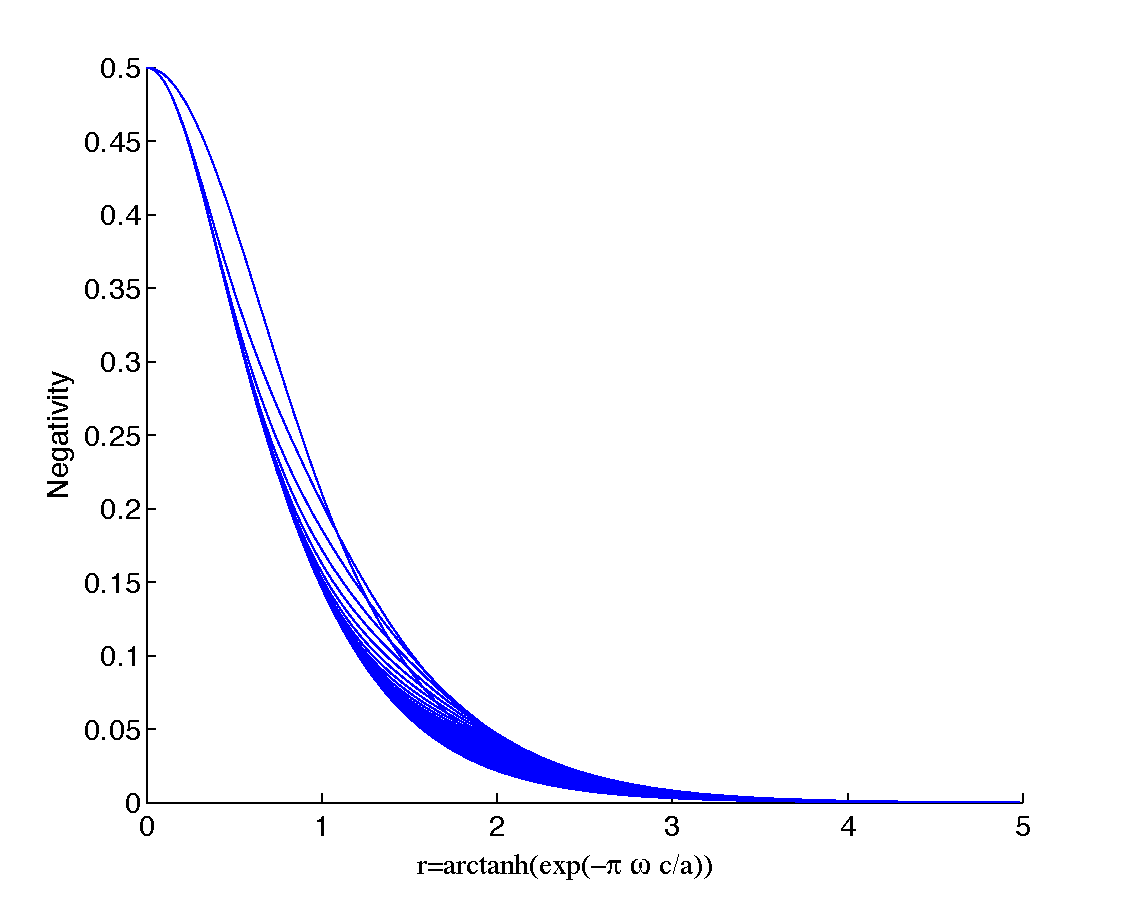
\includegraphics[width=.85\textwidth]{bundle}
\end{center}
\caption{Bundle of curves displaying the negativity for the bipartition AR for all values of $N$ as a function of the acceleration.}
\label{bundle}
\end{figure}

Figure \ref{bundle} shows the behaviour of negativity for all values of $N$, which is clearly similar for all cases no matter how many dimensions we are allowing for each mode. Despite this, negativity AR is slightly sensitive to dimension variations.

$\mathcal{N}^{AR}$ is shown in figure \ref{negaARcomp} as a function of $r$ for different values of $N$, comparing them with the case $N=1$. 
A very interesting result emerges here, for any pair of values for the maximum occupation number $N_1<N_2$ both negativity curves cross in a point $a=a_c(N_1,N_2)$. This means that for any finite value of the Hilbert space dimension there is a region $a<a_c(N_1,N_2)$ (low accelerations) in which entanglement is more degraded for higher dimension, and another region $a>a_c(N_1,N_2)$ (high accelerations)  in which entanglement is more degraded for lower dimension.
\begin{figure}[h]
\begin{center}
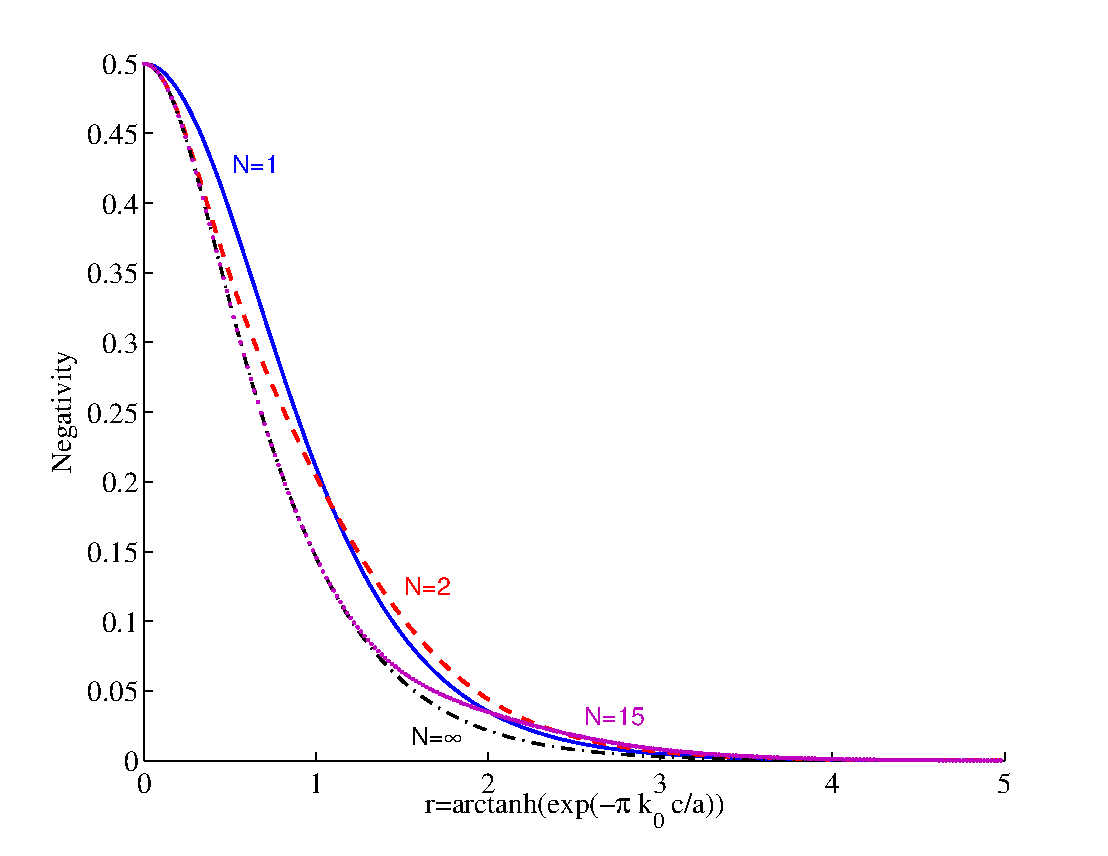
\includegraphics[width=.85\textwidth]{negaARcomp}
\end{center}
\caption{Same as fig. \ref{bundle} particularised for different values of the occupation number bound $N$ showing the existence of crossing points. To the right (left) of these points entanglement degrades less (more) for lesser $N$. Solid blue line $N=1$, dashed red line $N=2$, dotted purple line $N=15$, black dash-dotted line $N=\infty$.}
\label{negaARcomp}
\end{figure}

This disagrees the naive argument that higher dimension would lead to higher Unruh decoherence which is not necessarily true. Figure \ref{rcritical} shows the behaviour of $r_c(1,N)$ as $N$ grows. The crossing point with the negativity curve for $N=1$ grows as we consider larger $N$ curves. $r_c(N_1,N_2)$ is related with $a_c(N_1,N_2)$ by means of the relationship \eqref{defr1}.

\begin{figure}[h]
\begin{center}
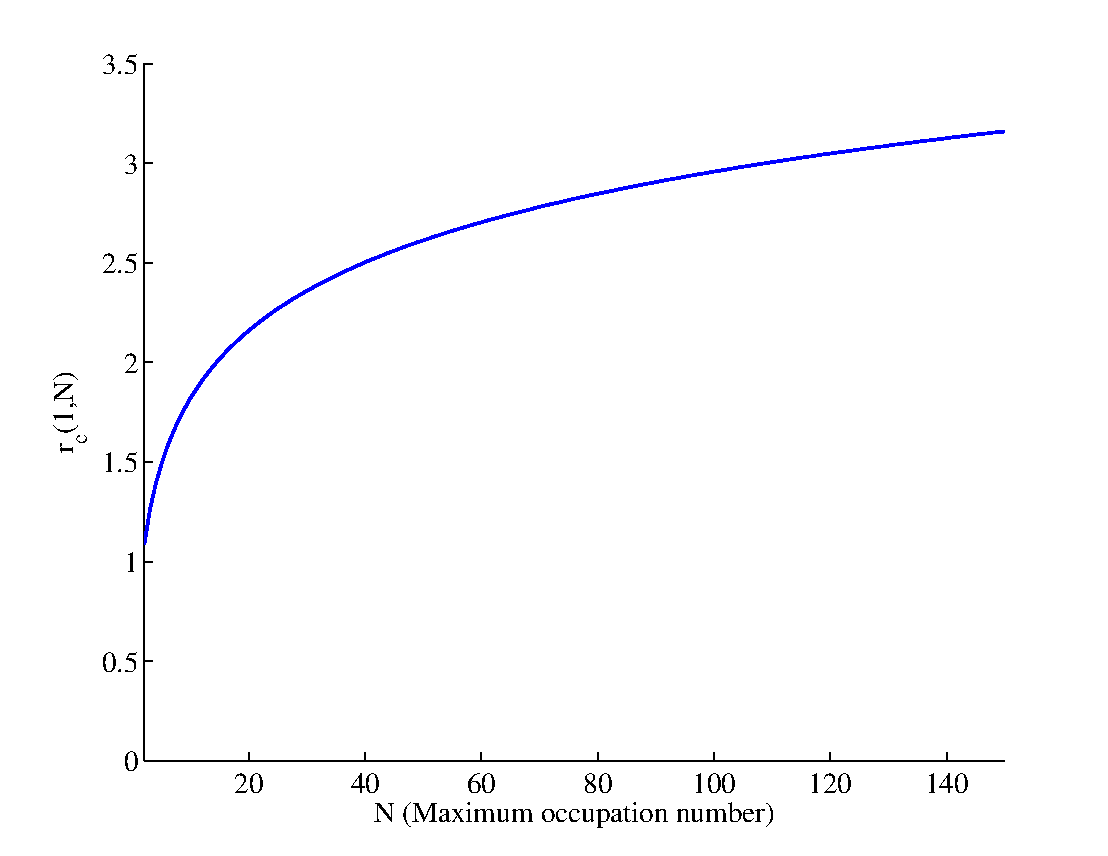
\includegraphics[width=.85\textwidth]{rcritical}
\end{center}
\caption{$r$ for which negativity curves for a bound $N$ cross the negativity curve for $N=1$. In the region above the curve entanglement degrades faster for $N=1$ than for $N>1$.}
\label{rcritical}
\end{figure}

For the limit $N_2\rightarrow\infty$,  $a_c(N_1,N_2)\rightarrow\infty$, which means that infinite dimension negativity is below all the finite dimensional curves.


\subsubsection{Bipartition Alice-AntiRob}

Excepting the diagonal elements corresponding to $\proj{10}{10}$ and $\proj{0N}{0N}$  (which form two $1\times1$ blocks themselves), the partial transpose of the density matrix $\rho^{\text{A}{\bar{\text{R}}}}$ \eqref{etaAaRs} has a $2\times2$ block structure in the basis $\{ \ket{0 n},\ket{1\, n+1}\}_{n=0}^{N-1}$ 
\begin{equation}\label{blocksbosAaR}
\frac{\tanh^{2n}r}{C(r)^2\cosh^2 r}
\left(\!\begin{array}{cc}
1 & \dfrac{\tanh r}{\cosh r}\sqrt{n+1}\\[3mm]
\dfrac{\tanh r}{\cosh r}\sqrt{n+1} & \dfrac{\tanh^2 r}{\cosh^2r}(n+2)
\end{array}\!\right).
\end{equation}
Hence, the eigenvalues of \eqref{etaAaRs} are
\begin{align}
\nonumber\lambda^{\pm}_n&\!=\!\frac{\tanh^{2n}r}{2C(r)^2\cosh^2 r}\Bigg[\!\left(1\!+\!(n\!+\!2)\frac{\tanh^2 r}{\cosh^2 r}\right)\left.\!\!\pm\sqrt{\!\left(1+(n+2)\frac{\tanh^2 r}{\cosh^2 r}\right)^2\!\!\!-\frac{4\tanh^2 r}{\cosh^2 r}}\!\right]_{n=0}^{N-1}\!\!\!\!,\nonumber\\*
\lambda_N&=\frac{1}{C(r)^2\cosh^4 r};\qquad\qquad \lambda_{N+1}=\frac{\tanh^{2N}r}{C(r)^2\cosh^2 r}.
\end{align}
Therefore, the negativity for this bipartition is always $0$, independently of the value of the acceleration parameter and the occupation number bound $N$.

From this results can be concluded that limiting the dimension has no effect in the creation or not of quantum correlations between Alice and AntiRob. As far as the field is bosonic, no entanglement is created in the CCA bipartitions of the system no matter how we limit the dimension of the Hilbert space.


\subsubsection{Bipartition Rob-AntiRob}

The partial transpose of the density matrix $\rho^{\text{R}{\bar{\text{R}}}}$  \eqref{etaRaRs} has a block structure. Namely, it is formed by $2N+1$ blocks whose dimension varies. In the following we will detailedly analyse the blocks.

\begin{enumerate}
\item First of all, we have $N+1$ blocks $\left\{M_D\right\}_{D=1}^{N+1}$  which are  endomorphisms that act in the subspace (of dimension $D$) expanded by the basis $B_{D}=\{\ket{mn}\}$ in which $m+n=D-1\le N$. 
\item Then we have $N$ more blocks $\left\{M'_D\right\}_{D=1}^N$ that  act in the subspace (of dimension $D$) expanded by the basis $B'_{D}=\{\ket{m'n'}\}$ in which $m'+n'=2N-D+1>N$. Notice that not all the possible $m'$ and $n'$ are allowed due to the limitation to the occupation number $m',n'\le N$.
\end{enumerate}

As an example which will perfectly clarify this construction, if $N=4$ there will be 9 blocks, $M_1,M_2,M_3,M_4,M_5, M'_4,M'_3,M'_2,M'_1$ each one is an endomorphism which acts in the subspace expanded by the bases
\begin{eqnarray}
\nonumber B_1&=&\left\{\ket{00}\right\},\\*
\nonumber B_2&=&\left\{\ket{01},\ket{10}\right\},\\*
\nonumber B_3&=&\left\{\ket{02},\ket{20},\ket{11}\right\},\\*
\nonumber B_4&=&\left\{\ket{03},\ket{30},\ket{12},\ket{21}\right\},\\*
\nonumber B_5&=&\left\{\ket{04},\ket{40},\ket{13},\ket{31},\ket{22}\right\},\\*
\nonumber B'_4&=&\left\{\ket{14},\ket{41},\ket{23},\ket{32}\right\},\\*
\nonumber B'_3&=&\left\{\ket{24},\ket{42},\ket{33}\right\},\\*
\nonumber B'_2&=&\left\{\ket{34},\ket{43}\right\},\\*
\nonumber B'_1&=&\left\{\ket{44}\right\}\\*
\end{eqnarray}
respectively.

In this fashion, the whole matrix is an endomorphism within the subspace R=$\bigoplus_{i=1}^{N+1} S_{i}\oplus\bigoplus_{j=1}^N S'_j$, being $S_{i}$ the subspace (of dimension $D=i$) expanded by the basis $B_{i}$ and $S'_j$ the subspace (of dimension $D=j$) expanded by the basis $B'_j$ .

The blocks $M_1,\dots,M_{N+1}$ and $M'_1,\dots,M'_{N}$ which form the matrix \eqref{etaRaRs} have the following form
\begin{equation}\label{blockss}
M_D=\left(\!
\begin{array}{cccccccc}
0  & a_1  & 0 & 0 & \cdots & \cdots& \cdots& 0 \\
a_1 & 0 & a_2 & 0 & \cdots & \cdots& \cdots & 0\\
0 & a_2 & 0 & a_3 & \cdots & \cdots& \cdots& 0\\
0 & 0 & a_3 &0 & a_4 & \cdots& \cdots& 0\\
0 & 0 & 0 &  \ddots &\ddots &  \ddots &\cdots& 0\\
\vdots  & \vdots  & \vdots  & \vdots  & \ddots  & \ddots  & \ddots  & \vdots \\
0 & 0 & 0 &  0 &\cdots&  \ddots &0& a_{D-1}\\
0 & 0 & 0 &  0 &0&  \dots &a_{D-1}& a_{D}\\
\end{array}\!\right).
\end{equation}

\begin{equation}
M'_D=\left(\!
\begin{array}{cccccccc}
0  & b_{1}  & 0 & 0 & \cdots & \cdots& \cdots& 0 \\
b_{1} & 0 & b_{2} & 0 & \cdots & \cdots& \cdots & 0\\
0 & b_{2} & 0 & b_{3} & \cdots & \cdots& \cdots& 0\\
0 & 0 & b_{3} &0 & b_{4} & \cdots& \cdots& 0\\
0 & 0 & 0 &  \ddots &\ddots &  \ddots &\cdots& 0\\
\vdots  & \vdots  & \vdots  & \vdots  & \ddots  & \ddots  & \ddots  & \vdots \\
0 & 0 & 0 &  0 &\cdots&  \ddots &0& b_{D-1}\\
0 & 0 & 0 &  0 &0&  \dots &b_{D-1}& b_{D}\\
\end{array}\!\right).
\end{equation}

The matrix elements $a_n$ and $b_n$ are defined as follows
\begin{align}
\nonumber a_{2l+1}&=\frac{(\tanh r)^{D-1}}{C(r)^2\cosh^2 r},\\*
\nonumber a_{2l}&=\sqrt{D-l}\,\sqrt{l}\frac{(\tanh r)^{D-2}}{C(r)^2\cosh^4r},\\*
\nonumber b_{2l+1}&=\frac{(\tanh r)^{2N-D+1}}{C(r)^2\cosh^2 r},\\*
 b_{2l}&=\sqrt{N+1-l}\,\sqrt{l+N-D+1}\frac{(\tanh r)^{2N-D}}{C(r)^2\cosh^4r}.
\end{align}
Notice that the elements are completely different when the value of the label $n$ is odd or even.

As the whole matrix is the direct sum of the blocks
\begin{equation}
\eta^{R \bar R}=\left(\bigoplus_{D=1}^{N+1} M_D\right) \oplus \left(\bigoplus_{D=1}^{N} M'_D\right),
\end{equation}
the eigenvalues and, specifically, the negative eigenvalues of $\eta^{R \bar R}$ would be the negative eigenvalues of all the blocks $M_D$ and $M'_D$  gathered togheter, which can be easily computed numerically.  Figure \ref{negaRAR} shows the behaviour of $\mathcal{N}^{\text{R}{\bar{\text{R}}}}$ with $r$ and for different values of $N$.
\begin{figure}[h]
\begin{center}
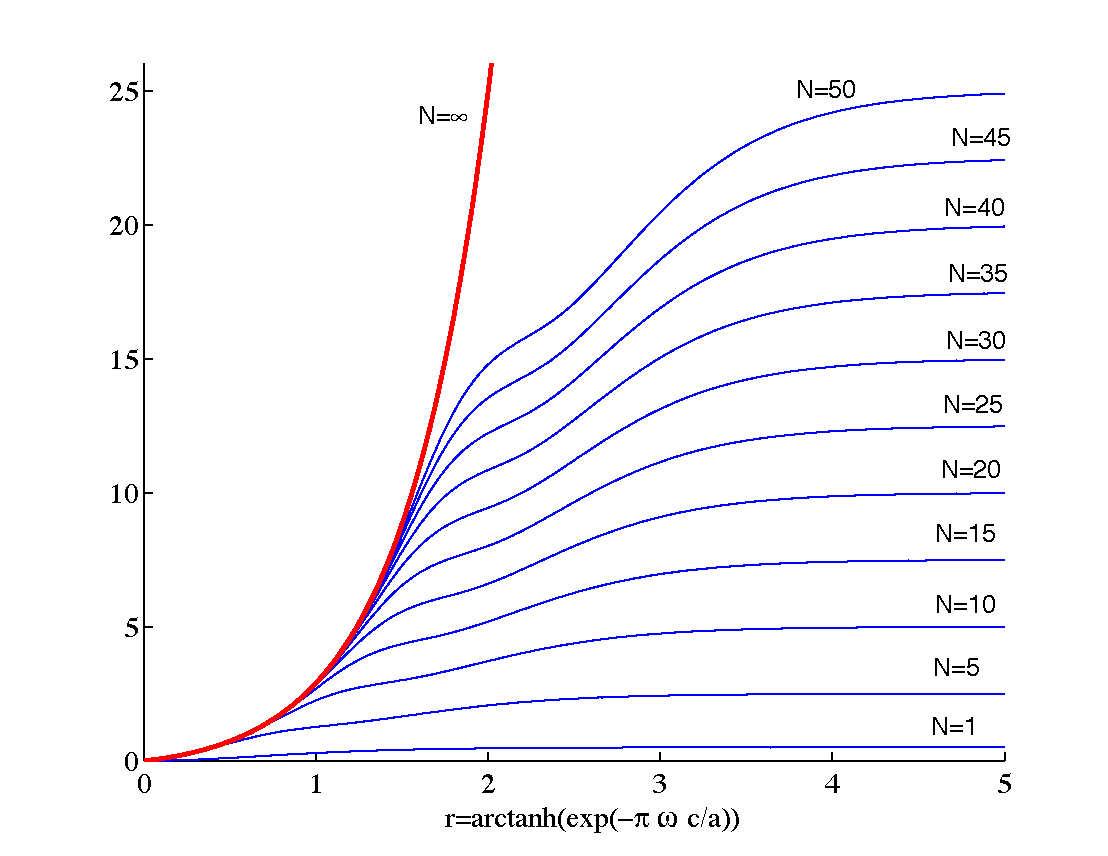
\includegraphics[width=.85\textwidth]{NegaRAR}
\end{center}
\caption{ Negativity $\text{R}{\bar{\text{R}}}$ for different values of $N$, showing the upper bound reached when $a\rightarrow\infty$. Negativity diverges when $a\rightarrow\infty$ only for $N\rightarrow\infty$.}
\label{negaRAR}
\end{figure}

We can now compare the finite $N$ bosonic case with their same dimension analog for fermions. Namely, a Grassmann scalar field (spinless fermion) has the same Hilbert space dimension as the scalar case with $N=1$, the relevant difference is the anticommutation of the field operators instead of the commutation which applies for bosons. On the other hand, scalars limited to $N=3$ and $N=2$ can be considered as two different analogs to the Dirac field as the former has the same Hilbert space dimension as Dirac modes and the latter would share the same possible maximum occupation number. 

This comparison can be seen in figures \ref{comparison1}, \ref{comparison2}. We see that the behaviour is similar (monotonic growth from zero to a finite limit for $a\rightarrow\infty$) but the functional dependence is still very different in both cases. Specifically, as $a$ increases the bosonic cases grow a higher entanglement between the modes of the field on both sides of the horizon than the same dimension fermionic analogs. 

\begin{figure}[h]
\begin{center}
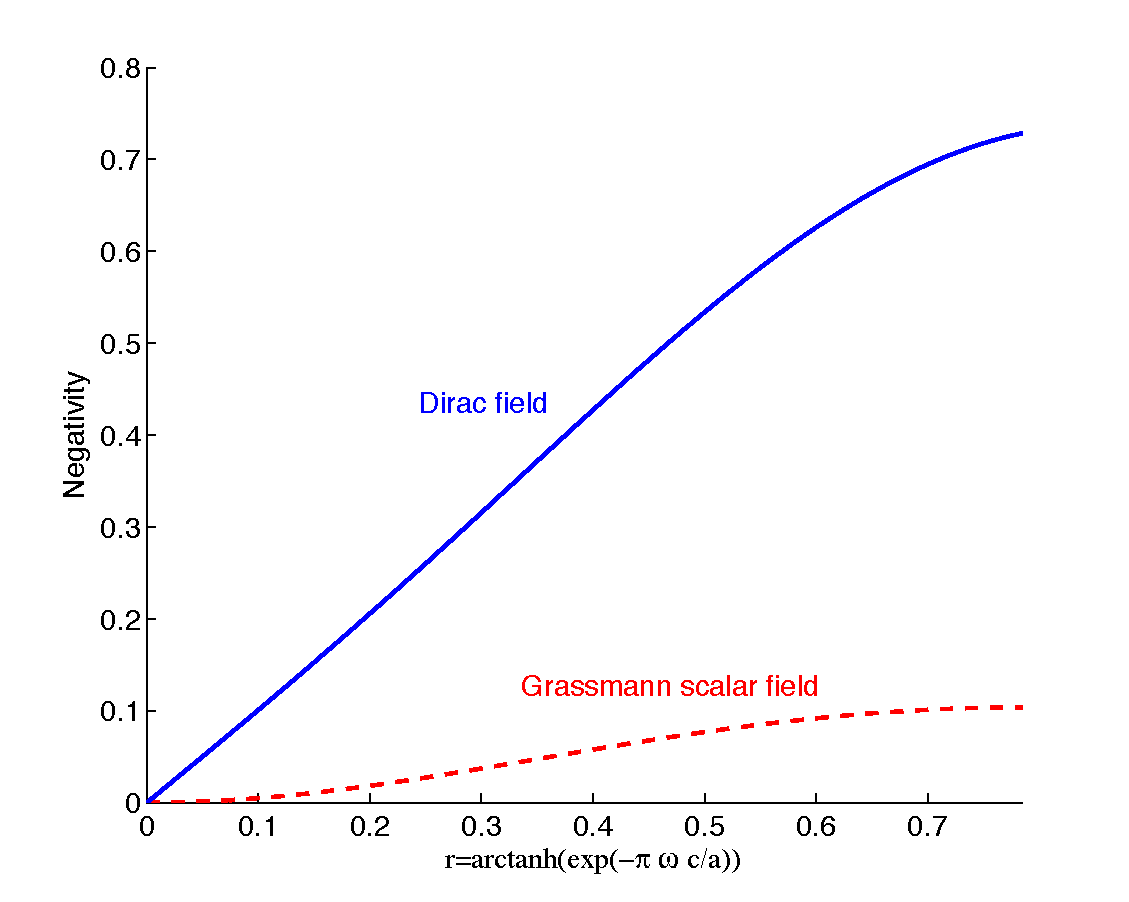
\includegraphics[width=.85\textwidth]{comparison1}
\end{center}
\caption{ Negativity of the bipartition $\text{R}{\bar{\text{R}}}$ for fermion fields. Grassmann scalar (red dashed line) and Dirac (blue solid line). Negativity upper bound is greater for the Dirac case as $\dim(\mathcal{H}_{\text{Dirac}})>\dim(\mathcal{H}_{\text{Grassmann}})$. Notice that here $r=\operatorname{atan}(e^{-\pi k_0/a})$ instead of the hyperbolic tangent and therefore $r\rightarrow\pi/4\Rightarrow a\rightarrow\infty$. }
\label{comparison1}
\end{figure}
\begin{figure}[h]
\begin{center}
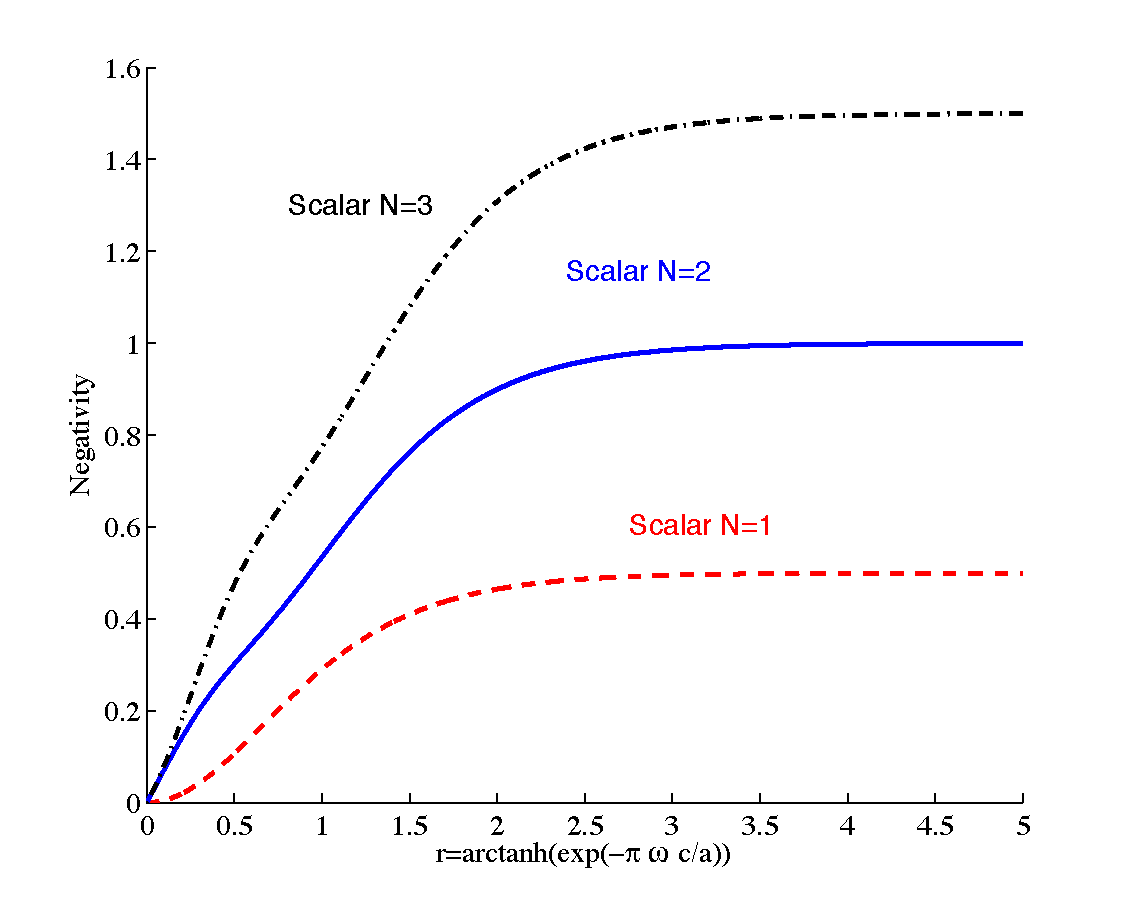
\includegraphics[width=.85\textwidth]{comparison2}
\end{center}
\caption{ Same as fig. \ref{comparison1} but for bounded occupation number scalar fields. $N=1$ (red dashed line) is dimensionally analogous to the Grassmann scalar case. $N=3$ (black dash-dotted line) is dimensionally analogous to the Dirac case. $N=2$ (blue solid line) is analogous to the Dirac field in maximum occupation number.}
\label{comparison2}
\end{figure}

This clearly shows another important difference between fermionic and bosonic fields. Pauli exclusion principle prevents the total degradation of fermionic  entanglement in CCA bipartitions, whereas, conversely, impedes entanglement creation between $\text{R}{\bar{\text{R}}}$.




\subsection{Mutual information}\label{mutualsec}

Mutual information accounts for correlations (both quantum and classical) between two different partitions of a system (see section \ref{mutusec}). It is defined as
\begin{equation}\label{mutualdef}
I_{AB}=S_A+S_B-S_{AB},
\end{equation}
where $S_A$, $S_B$ and $S_{AB}$ are respectively the Von Neumann entropies for the individual subsystems $A$ and $B$ and for the joint system $AB$.

To compute the mutual information  for each bipartition we will need the eigenvalues of the corresponding density matrices. We shall go through all the process detailedly in the lines below.

\subsubsection{Alice-Rob Bipartition}

Excepting the element $\proj{0N}{0N}$ (which forms a $1\times1$ block itself) the density matrix for the system Alice-Rob \eqref{rhoars1} consists on $N$ $2\times2$ blocks in the basis $\{\ket{0 n},\ket{1\, n+1}\}_{n=0}^{N-1}$ which have the form
\begin{equation}
\frac{\tanh^{2n}r}{C_N(r)^2\cosh^2r }
\left(\!\begin{array}{cc}
1 & \dfrac{\sqrt{n+1}}{\cosh r}\\
\dfrac{\sqrt{n+1}}{\cosh r} & \dfrac{n+1}{\cosh^2r}
\end{array}\!\right).
\end{equation}
Hence, the eigenvalues of \eqref{rhoars1} are
\begin{eqnarray}\label{eigAR}
\nonumber\lambda_n&=&\left.\frac{\tanh^{2n}r}{C_N(r)^2\cosh^2r}\left(1+\frac{n+1}{\cosh^2 r}\right)\right|_{n=0}^{N-1}\\*
\lambda_N&=&\frac{\tanh^{2N} r}{C_N(r)^2\cosh^2r},
\end{eqnarray}
along with $N$ identically zero eigenvalues.

\subsubsection{Alice-AntiRob Bipartition}

Except from the diagonal element corresponding to $\proj{00}{00}$  (which forms one $1\times1$ block itself) the density matrix for the system Alice-AntiRob \eqref{rhoa-rs1} consists on $(N-1)$ $2\times2$ blocks in the basis $\{\ket{0 n},\ket{1\, n-1}\}_{n=1}^N$ which have the form
\begin{equation}
\frac{\tanh^{2n}r}{C_N(r)^2\cosh^2r}
\left(\!\begin{array}{cc}
1 & \dfrac{\sqrt{n}}{\sinh r} \\
\dfrac{\sqrt{n}}{\sinh r} & \dfrac{n}{\sinh^2 r}\\
\end{array}\!\right).
\end{equation}
Therefore the eigenvalues of \eqref{rhoa-rs1} are
\begin{eqnarray}\label{eigAaR}
\lambda_n&=&\left.\frac{\tanh^{2n}r}{C_N(r)^2\cosh^2r}\left(1+\frac{n}{\sinh^2r}\right)\right|_{n=0}^{N},
\end{eqnarray}
along with $N$ identically zero eigenvalues.


\subsubsection{Rob-AntiRob Bipartition} 


The density matrix for Rob-AntiRob  \eqref{rhor-rs1} consists in the direct sum of two blocks 
\begin{equation}\label{newdoe}
\rho^{\text{R}{\bar{\text{R}}}}=X\oplus Y
\end{equation}
of dimensions $\dim(X)=N+1$, $\dim(Y)=N$.
The matrix elements of $X$ and $Y$ are
\begin{equation}
X_{ij}=\frac{(\tanh r)^{i+j-2}}{C_N(r)^2\cosh^2r }\qquad Y_{ij}=\sqrt{i}\sqrt{j} \frac{(\tanh r)^{i+j-2}}{C_N(r)^2\cosh^4r}
\end{equation}
in the bases $\left\{\ket{nn}\right\}_{n=0}^{N}$ and $\left\{\ket{n+1\,n}\right\}_{n=0}^{N-1}$ respectively.

It is easy to see that $\operatorname{rank}(X)=\operatorname{rank}(Y)=1$. This means that all the eigenvalues of  \eqref{rhor-rs1} are zero  except for two of them, which we can readily compute
%\begin{eqnarray}\label{eigRaR0}
%\nonumber\lambda^{\text{R}{\bar{\text{R}}}}_{\Theta_1}&=&\sum_{n=0}^{N}\frac{\tanh^{2n}r}{2\cosh^2r}\\*
%\lambda^{\text{R}{\bar{\text{R}}}}_{\Theta_2}&=&\sum_{n=0}^{N-1}\frac{(n+1)\tanh^{2n}r}{2\cosh^4r}
%\end{eqnarray}
\begin{equation}\label{eigRaR}
\lambda^{\text{R}{\bar{\text{R}}}}_{X}=\frac{D_N^0(r)}{C(r)^2}\qquad\lambda^{\text{R}{\bar{\text{R}}}}_{Y}= \frac{D_N^1(r)}{C(r)^2},
\end{equation}
where $D_N^0(r)$ and $D_N^1(r)$ are given by \eqref{S1} and \eqref{S2}.


\subsubsection{Von Neumann entropies for each subsystem and mutual information}

To compute the Von Neumann entropies we need the eigenvalues of every bipartition and the individual density matrices. The eigenvalues of $\rho^{AR}$, $\rho^{A\bar R}$, $\rho^{\text{R}{\bar{\text{R}}}}$ are respectively \eqref{eigAR}, \eqref{eigAaR} and \eqref{eigRaR}.

The eigenvalues of the individual systems density matrices can be directly read from \eqref{Robpartial}, \eqref{ARobpartial} and \eqref{AlicedeAliceRob} since $\rho^R$, $\rho^{\bar R}$ and $\rho^A$ have diagonal forms in the Fock basis. The Von Neumann entropy for a partition $B$ of the system is $S=-\tr(\rho\log_2\rho)$. Therefore their entropies are
\begin{align}\label{entropARaR}
\nonumber S_{R}&=-\sum_{n=0}^{N}\frac{\tanh^{2n}r}{C_N(r)^2\cosh^2r}\left[1+\frac{n}{\sinh^2r}\right]\log_2\left[\frac{\tanh^{2n}r}{C_N(r)^2\cosh^2r }\left(1+\frac{n}{\sinh^2r}\right)\right],\\*
\nonumber S_{\bar R}&=-\sum_{n=0}^{N-1}\frac{\tanh^{2n}r}{C_N(r)^2\cosh^2r}\left[1+\frac{n+1}{\cosh^2r}\right]\log_2\left[\frac{\tanh^{2n}r}{C_N(r)^2\cosh^2r }\left(1+\frac{n+1}{\cosh^2r}\right)\right],\\*
\nonumber&-\frac{\tanh^{2N}r}{C_N(r)^2\cosh^2r }\log_2\left(\frac{\tanh^{2N}r}{C_N(r)^2\cosh^2r}\right)\\*
S_A&=2\log_2\left[C_N(r)\right]-\frac{1}{C_N(r)^2}\sum_{i=0,1}D^i_N(r)\log_2\left[D^i_N(r)\right].
\end{align}

We obtain a universal result which relates the entropies of the different bipartitions of the system, 
\begin{equation}
S_{AR}=S_{\bar R},\qquad S_{A\bar R}=S_R,\qquad S_{\text{R}{\bar{\text{R}}}}= S_A.
\end{equation}  
These results can be summarised in the expression
\begin{equation}
S_{IJ}=S_K,
\end{equation}
where $I,J$ and $K$ labels represent different subsystems. Whichever values $I\neq J\neq K$ will satisfy the identity. This is also true for standard scalar fields, Grassmann scalar fields (spinless fermions) and Dirac fields. These relationships are completely universal, being independent of statistics and dimension, and reflect a fundamental aspect of Unruh decoherence in terms of the entropy of the partial systems, namely,  the way in which the entropy of the bipartitions behaves as acceleration increases  is not independent from the way the individual entropies do. 

The mutual information for all the possible bipartitions of the system will be
\begin{eqnarray}
\nonumber I_{AR}&=&S_A+S_R-S_{A R}=S_A+S_R -S_{\bar R},\\*
\nonumber I_{A\bar R}&=&S_A+S_R-S_{A\bar R}=S_A+ S_{\bar R}-S_R,\\*
\nonumber I_{\text{R}{\bar{\text{R}}}}&=& S_R+S_{\bar R}-S_{\text{R}{\bar{\text{R}}}}=S_A+ S_{\bar R}+S_R.
\end{eqnarray}  

The first notable difference from the standard bosonic field is that we do not obtain here the conservation law of the mutual information for the system Alice-Rob and Alice-AntiRob, instead
\begin{equation}\label{noconservationbos}
 I_{AR} + I_{A\bar R}=2S_{A},
\end{equation}
where for any finite $N$, $S_A$ goes to zero when $a\rightarrow\infty$. Only in the limit of $N\rightarrow\infty$ where $S_{A}\rightarrow 1$  $\forall a$ the conservation law is restored. 

Figure \ref{MutuARAAR1} shows  the mutual information tradeoff of the systems AR and $\text{A}{\bar{\text{R}}}$ from $N=1$ to $N=10^4$, along with the limit $N\rightarrow\infty$ in which the conservation law is fulfilled for all values of $a$. 
\begin{figure}[h]
\begin{center}
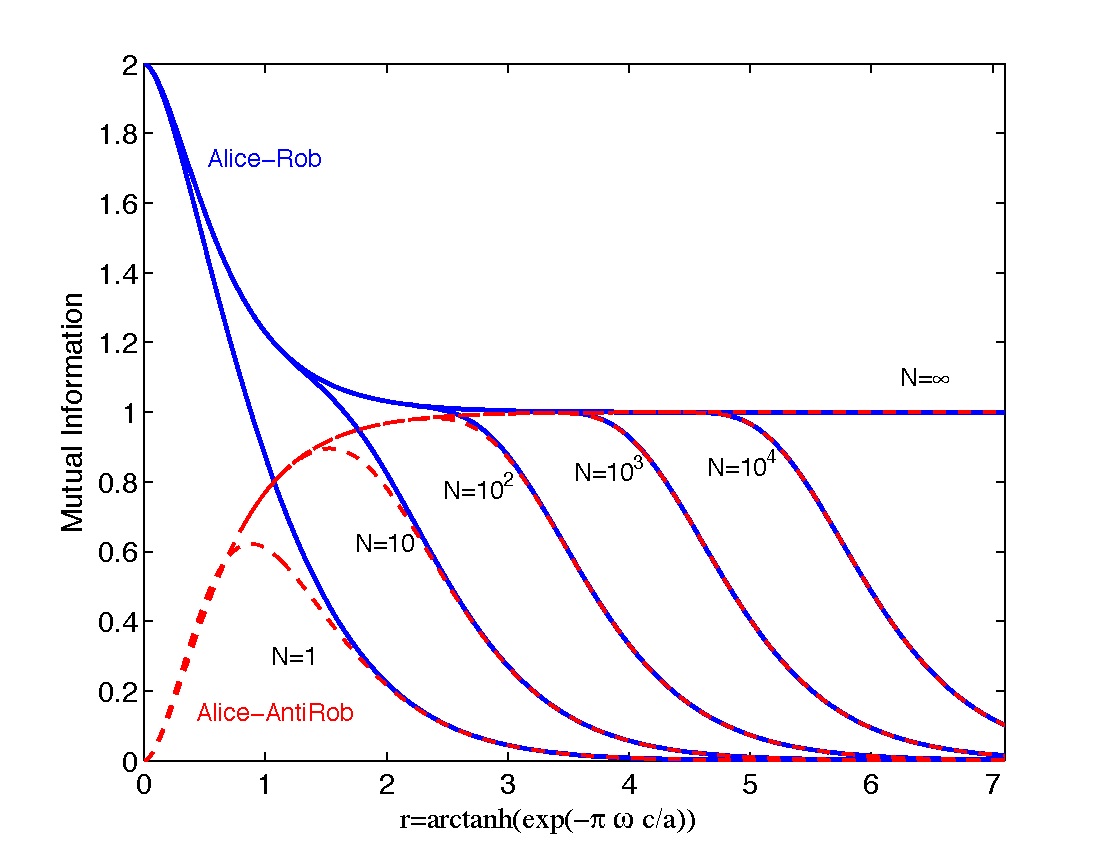
\includegraphics[width=.85\textwidth]{MutuARAAR1}
\end{center}
\caption{ Mutual information for the systems Alice-Rob (blue continuous lines) and Alice-AntiRob (red dashed lines) as the acceleration parameter varies. Several values of $N$ are plotted along with the $N=\infty$ case. A conservation law is satisfied until acceleration reaches a critical value which is displaced to the right logarithmically as $N$ increases.}
\label{MutuARAAR1}
\end{figure}


As it can be seen in Figure \ref{conserva} the largest deviation from the conservation law is obtained for $N=1$. As it is shown in the Figure, for a given $N$ the conservation law is fulfilled until the acceleration reaches a critical value $a=a_{l}$, then correlations go rapidly to zero. This critical value increases logarithmically with $N$. 

\begin{figure}[h]
\begin{center}
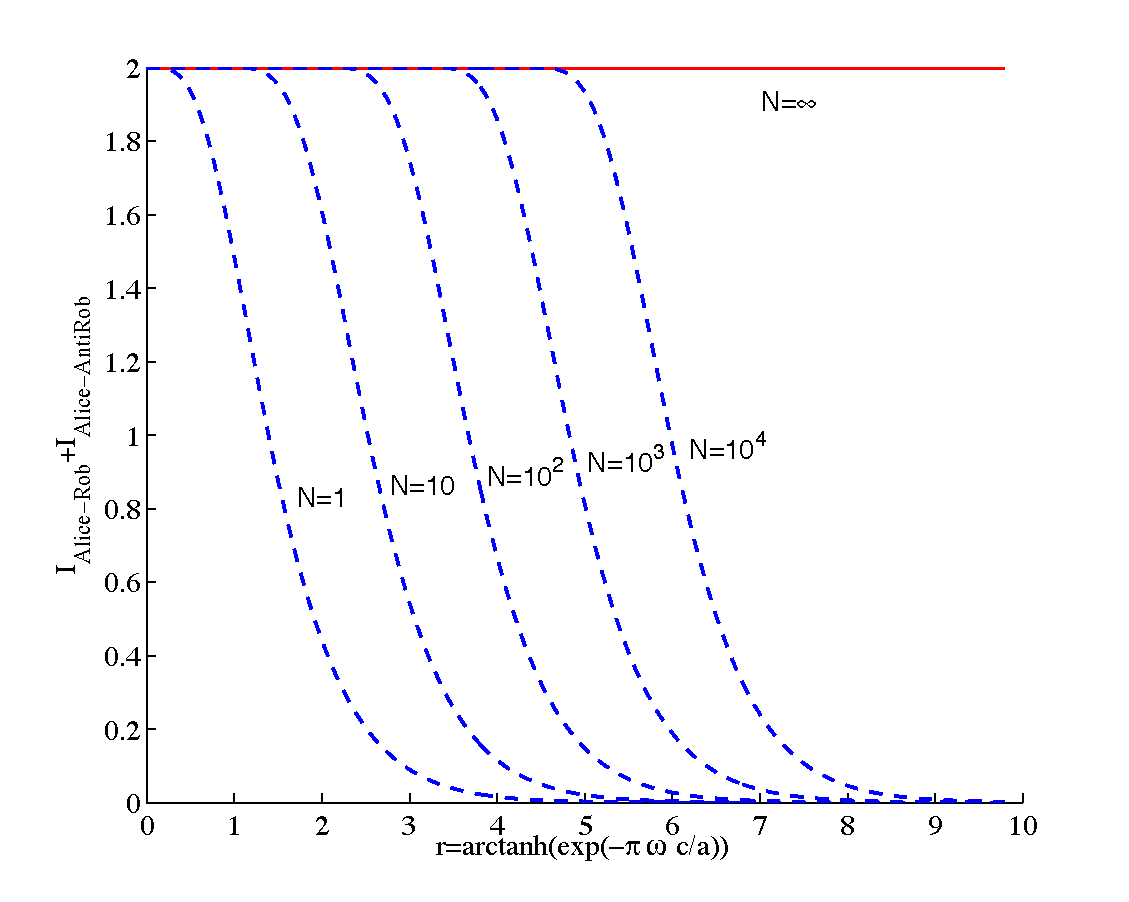
\includegraphics[width=.85\textwidth]{conserva}
\end{center}
\caption{ Violation of mutual information conservation law for the systems AR and $\text{A}{\bar{\text{R}}}$. The conservation law is fulfilled until $a$ reaches a critical value which is logarithmically displaced to the right as $N$ increases. The conservation law is completely restored when $N\rightarrow\infty$.}
\label{conserva}
\end{figure}



We showed above that quantum correlations between AR are quickly lost as $a$ increases for all $N$  and no entanglement is created between $\text{A}{\bar{\text{R}}}$. This means that for the high acceleration regime (where quantum entanglement vanishes) classical correlations dominate mutual information. Therefore, what we learn from mutual information in this regime is the behaviour of purely classical\footnote{There might be also quantum discord \cite{Discord}, but it is irrelevant in our analysis since our interest here is to distinguish entanglement from the rest of correlations.} correlations which are usually very difficult to be studied separately from entanglment.

For the scalar field we have seen that, conversely to fermionic fields,  limiting the dimension produces boundary effects which make classical correlations go to zero. Here, conservation of these correlations for all values of $a$ requires infinite dimension. In other words, finite dimensions schemes kill classical correlations as Rob accelerates in the bosonic case.

One would expect something similar for fermions since their states are naturally of finite dimension. Hence, similar `border effects' in classical correlations should appear in the same fashion as for bosons. Despite this fact, mutual information for fermions does not vanish. The explanation for this difference between bosons and fermions comes from fermionic quantum correlations. As shown in chapter \ref{etanthrough}, there is a conservation law for fermionic quantum entanglement 
\begin{equation}\label{connetfer}
\mathcal{N}^{AR}_{\text{fermions}}+\mathcal{N}^{\text{A}{\bar{\text{R}}}}_{\text{fermions}}=\frac12.
\end{equation}
Since classical correlations for the finite dimensional case eventually go to zero, quantum correlations rule mutual information behaviour for fermions. Therefore, it can be concluded that  the conservation law for the mutual information for fermions must be strongly related with the conservation of the fermionic entanglement which has its origin in statistics. 

We can conclude then that the origin of the universal mutual information conservation law is different for fermions and bosons. On one hand, for bosons, it appears as a classical correlations conservation law. On the other hand, for fermions, this law reflects a quantum correlations conservation. This can also explain why mutual information behaves so similarly to negativity for fermions as it was obtained in chapter \ref{etanthrough}.  

To finish this work and complete the analysis of mutual information let us show in Figure \ref{GOREBADA}  how the behaviour of $I_{\text{R}{\bar{\text{R}}}}$ changes as $N$ is increased and how the divergent limit is obtained when $N\rightarrow\infty$. The results about mutual information here are coherent with the thorough analysis of the correlations for the $\text{R}{\bar{\text{R}}}$ bipartition performed above when we analysed negativity.

\begin{figure}[H]
\begin{center}
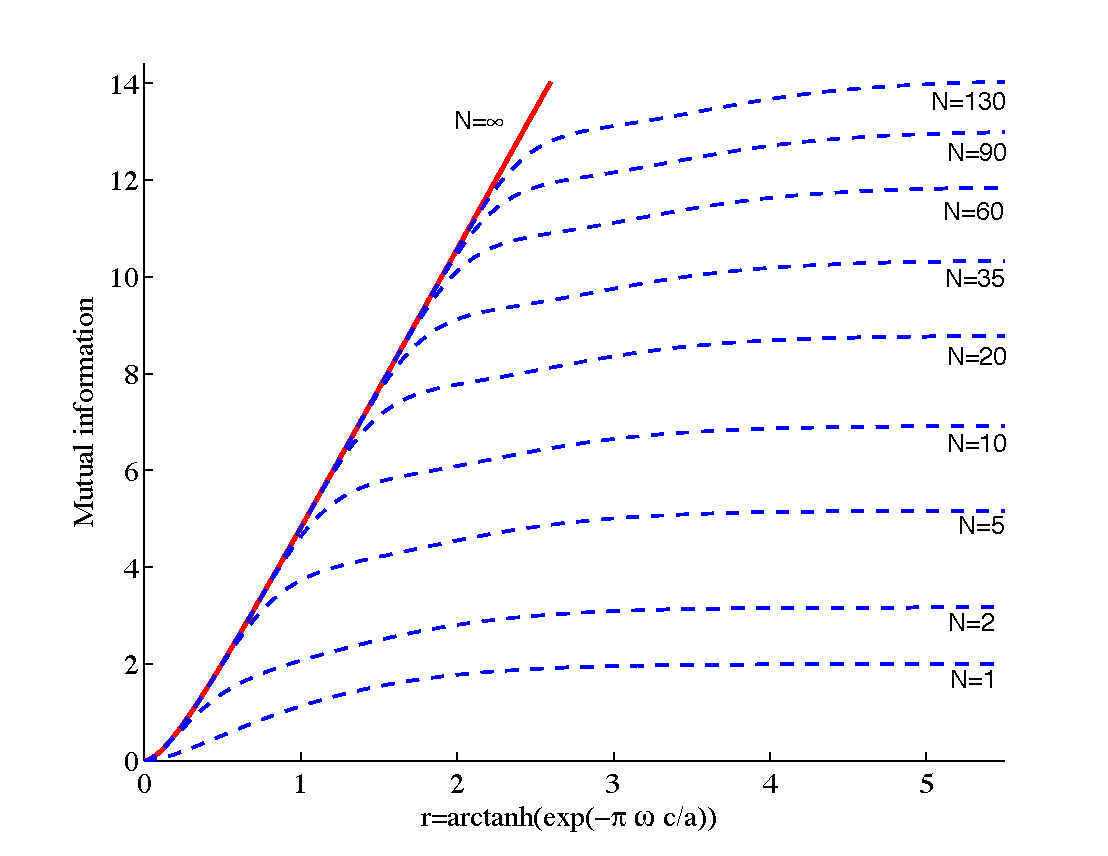
\includegraphics[width=.85\textwidth]{MutualRAR}
\end{center}
\caption{Mutual information for the system R-${\bar{\text{R}}}$ as acceleration varies for different values of $N$. Only for $N\rightarrow\infty$ Mutual information diverges.}
\label{GOREBADA}
\end{figure}

\section{Discussion}\label{conclusions}

In this chapter we answer the question of the actual impact of Fock space dimensionality on the Unruh entanglement degradation phenomena. To do so, we have studied the dimensional dependence of scalar field correlations when one observer is non-inertial. With this end in sight we have built a scalar field entangled state in which we have imposed a maximum occupation number $N$ for Rindler modes.

We have shown that the entanglement for AR and $\text{A}{\bar{\text{R}}}$ is only slightly influenced by $N$. In other words, the qualitative behaviour (quick loss of entanglement for AR as shown in Figure \ref{bundle} and no entanglement creation for the system $\text{A}{\bar{\text{R}}}$) is the same for finite and infinite $N$. This again points to the argument given in previous chapters that it is statistics and not dimensionality that conditions the behaviour of correlations in the presence of horizons.

However, we have shown that AR entanglement is sensitive to variations of $N$. This opposes what we found for fermions, whose correlations are completely insensitive to Hilbert space dimension variations (for example going from Grassmann scalars to Dirac fields).

In previous works we found a universal behaviour for the fermionic entanglement of the bipartition AR. Specifically the functional form of the negativity was exactly the same; independent of the maximally entangled state selected, the spin of the field, and the number of modes considered going beyond SMA. In all the cases Unruh decoherence degrades fermionic entanglement exactly in the same way. Here we see that for bosons this universality principle does exist but it is not as strong due to the sensitivity of AR to dimension changes. 

We have also seen that lesser $N$ does not necessarily imply faster entanglement degradation. Instead, we have shown that for two different finite values of $N$, namely $N_1<N_2$ there is a region $a<a_c$ in which entanglement is more degraded for $N_2$ and another region $a>a_c$ in which entanglement is more degraded for $N_1$. In other words, for high accelerations, higher dimension means less entanglement degradation by Unruh effect. This result clashes again with the extended idea that lesser dimension would protect correlations better than higher dimension, one misconception that after all this research should be banished from the explanation of these phenomena.

We have also showed that, since $a_c$ shifts to the right as $N$ is increased, in the limit $N\rightarrow\infty$, $a_c\rightarrow\infty$, so that entanglement is more degraded for the infinite dimensional case than for any finite $N$ whatever the value of the acceleration.

It is remarkable that there is no entanglement tradeoff in the CCA bipartitions even for finite dimension; no entanglement appears in the bipartition $\text{A}{\bar{\text{R}}}$ whatever the dimension limit $N$. This reflects again that the differences between fermions and bosons have nothing to do with the finite dimensionality, but with the different statistics. 

Concerning mutual information, we have shown that the conservation law found for scalar fields in chapter \ref{etanthrough} for the systems AR and $\text{A}{\bar{\text{R}}}$ is violated for finite values of $N$. We have obtained that for a finite $N$ the conservation law is fulfilled until acceleration reaches a critical value, in which correlations quickly drop. This critical value grows logarithmically with $N$, which means that the conservation law is satisfied for all $a$ when $N\rightarrow\infty$. Therefore, the violation of this conservation law can be associated with the boundary effects of imposing a dimensional limit. It is important to observe that in the bosonic case, mutual information is mainly accounting for classical correlations since quantum entanglement in the bosonic case are quickly lost as $a$ increases.

One could expect something similar in the fermionic case since fermions have a limited dimension Hilbert space for each mode. However, they lack these boundary effects. This big difference between fermions and bosons is related with the conservation of quantum entanglment in the $a\rightarrow\infty$ for fermions: in the high acceleration regime fermionic entanglement does not die (unlike the bosonic case) and therefore, for fermions, mutual information is accounting for quantum entanglement. This entanglement satisfies itself a conservation law \eqref{connetfer} which is `inherited' by mutual information. This also explains the similitude between mutual information and negativity behaviour for fermions found in chapter \ref{etanthrough}.

The conclusion here is that the universal conservation law for mutual information is found for both fermions and bosons, however the nature of this conservation is completely different in each case. For bosons it is due to classical correlations conservation, whereas for fermions it is due to quantum entanglement conservation. This illustrates once again that statistics is a paramount feature in order to explain how correlations behave in the presence of horizons.

The dimension of the Fock space has the largest impact in the behaviour of correlations between regions I and II separated by the horizon. Comparing the limited dimension scalar fields with their fermionic analogs we have found that the behaviour of correlations $\text{R}{\bar{\text{R}}}$ is somewhat similar for bosons and fermions and mainly ruled by the dimensionality of the Hilbert space. For both fermionic and bosonic fields, entanglement is always created between $\text{R}{\bar{\text{R}}}$ reaching a maximum value when $a\rightarrow\infty$ for any finite dimension.

The scalar cases of finite $N$ present, important differences compared with their fermionic Fock space dimensional analogs (namely $N=1$ is analogous to the Grassmann scalar case and $N=2,3$ to the Dirac field case). In the infinite acceleration limit, scalar states entanglement created between I and II modes is greater than in the fermionic case.

This implies that, regarding correlations between Rob and AntiRob modes, the effect of statistics is the opposite to what happened for the CCA bipartitions. Here bosonic correlations reach higher values than their corresponding fermionic analogs. 

